\chapter{Design and Implementation}\label{implement}

    In this chapter, the implementation details will be explained in many aspects, including Java Native Interface,
    human detection, and distance calculation.

    \section{Preparation}
        This application is implemented on the Android Operating System,
        and the target Software Development Kit (SDK) version is set at level 29, namely Android Q.
        This application is compiled and built by Android Studio version 3.5.3,
        and CMake is used for compiling C++ library with C++ version 11.
        Furthermore, OpenCV version 4.4.0, which is built as shared library, is used for image processing and object detection.
        For object detection model, there are 2 models are used: You Only Look Once and MobileNet SSD.

    \section{Java Native Interface}
        Implementation is divided into 3 layers.
            The first layer is an application layer, which is written in Java.
                This Layer mainly interacts with a user, checks permissions, and communicates with Java Native Interface (JNI).
                In addition, this layer also handle I/O implementation such as camera, file, and storage.
            The second layer is JNI, which is written in C and C++.
                JNI layer performs 2 main tasks.
                    The fist task is being an intermediate connection between the application layer and a library layer.
                    The second task is loading native shared libraries, which is compiled by a Native Development Kit (NDK).
            The last layer is the library layer, which is written in C++.
                This layer performs calculation tasks, including Deep Neural Network and distance calculation.

        However, Deep Neural Network and distance calculation can be implemented in the application layer,
        According to Android Developer Guide \cite{ANDROID-01},
        Native Development Kit (NDK) is recommended for compiling C and C++ coode into native library,
        which is able to achieve a higher performance.
        Thus, executing both tasks in the library layer gains a better performance.
        Furthermore, there are 2 advantages of implementing JNI.
            The first advantage is reducing JNI calling. Performing both tasks in an application layer have to call JNI methods many times,
                and this is expensive and cost an overhead.
                Thus, implementing JNI manually reduces the number of JNI calls.
            The second advantage is memory management. C++ is able to access values in the memory by using a pointer.
                Thus, values can be directly accessed without copying.

    \section{Human Detection}
        % Intro to detection
        There are 3 main processes is implemented to determine social distancing violation from the image and video.

        The first process is pre-processing the given image, video, or video stram.
        The given video will be extracted into an array of images.
        Then, images will be converted into Bitmap and Mat format with RGBA colour model respectively.
        After that, colour will be converted, which depends on a detection model.
        As mentioned in section 4.1, there are 2 detection models are used for detecting humans in the given picture and video: YOLO model and MobileNet SSD model.
        Colour will be converted to RGB if the detection model is YOLO,
        while MobileNet SSD requires BGR colour model.

        The second process is object detection.
        Detection models are setup and configured differently before processing images.
        First of all, YOLO is used with Darknet, which is an open source neural network framework,
            while MobileNet SSD. MobileNet is used with Caffe framework.
        Then, threshold will be set for determining the confidence level of the detected object.
            The confidence level threshold of YOLO model will be set to 0.5 or 50 percent.
            In other words, the detected object will be rejected if YOLO model cannot guarantee that a detected object is human,
            and its confidence level is lower than 50 percent.
            In contrast, The confidence level threshold of MobileNet SSD model will be set to 0.3 or 30 percent.
            Because of MobileNet SSD model has a lower ability to detect an object, the confidence threshold is set to be lower.

        After models are setup and configured, the image will be processed in 5 steps.
        For the first step, pre-processed image will be convert to input blob by passing Mat image to $blobFromImage()$ function with scale factor.
            Blob will be used for the forward propagation in the neural network.
        Secondly, blob will be passed to the network through $forward()$ function, and a list of detected boxes


\begin{lstlisting}
    for i:=maxint to 0 do
    begin
    { do nothing }
    end;
    Write('Case insensitive ');
    Write('Pascal keywords.');
\end{lstlisting}


        % Load and model configuration

        The first model is You Only Look Once (YOLO).
            YOLO is used with Darknet, which is an open source neural network framework.
            To determine the confidence level of the detected object, threshold is set to 0.5.
            In other words, the detected object will be rejected if the confidence level of the detected object is lower than 0.5.
        The second model is MobileNet SSD. MobileNet is used with Caffe framework.
            The confidence threshold of MobileNet SSD will be set to 0.3.
            The confidence threshold is set to be lower than YOLO because MobileNet SSD has a lower ability to detect an object.
            In other words, a few number of poeple will be detected if threashold is set to 0.5.

        \begin{figure}[!ht]
            \centering
            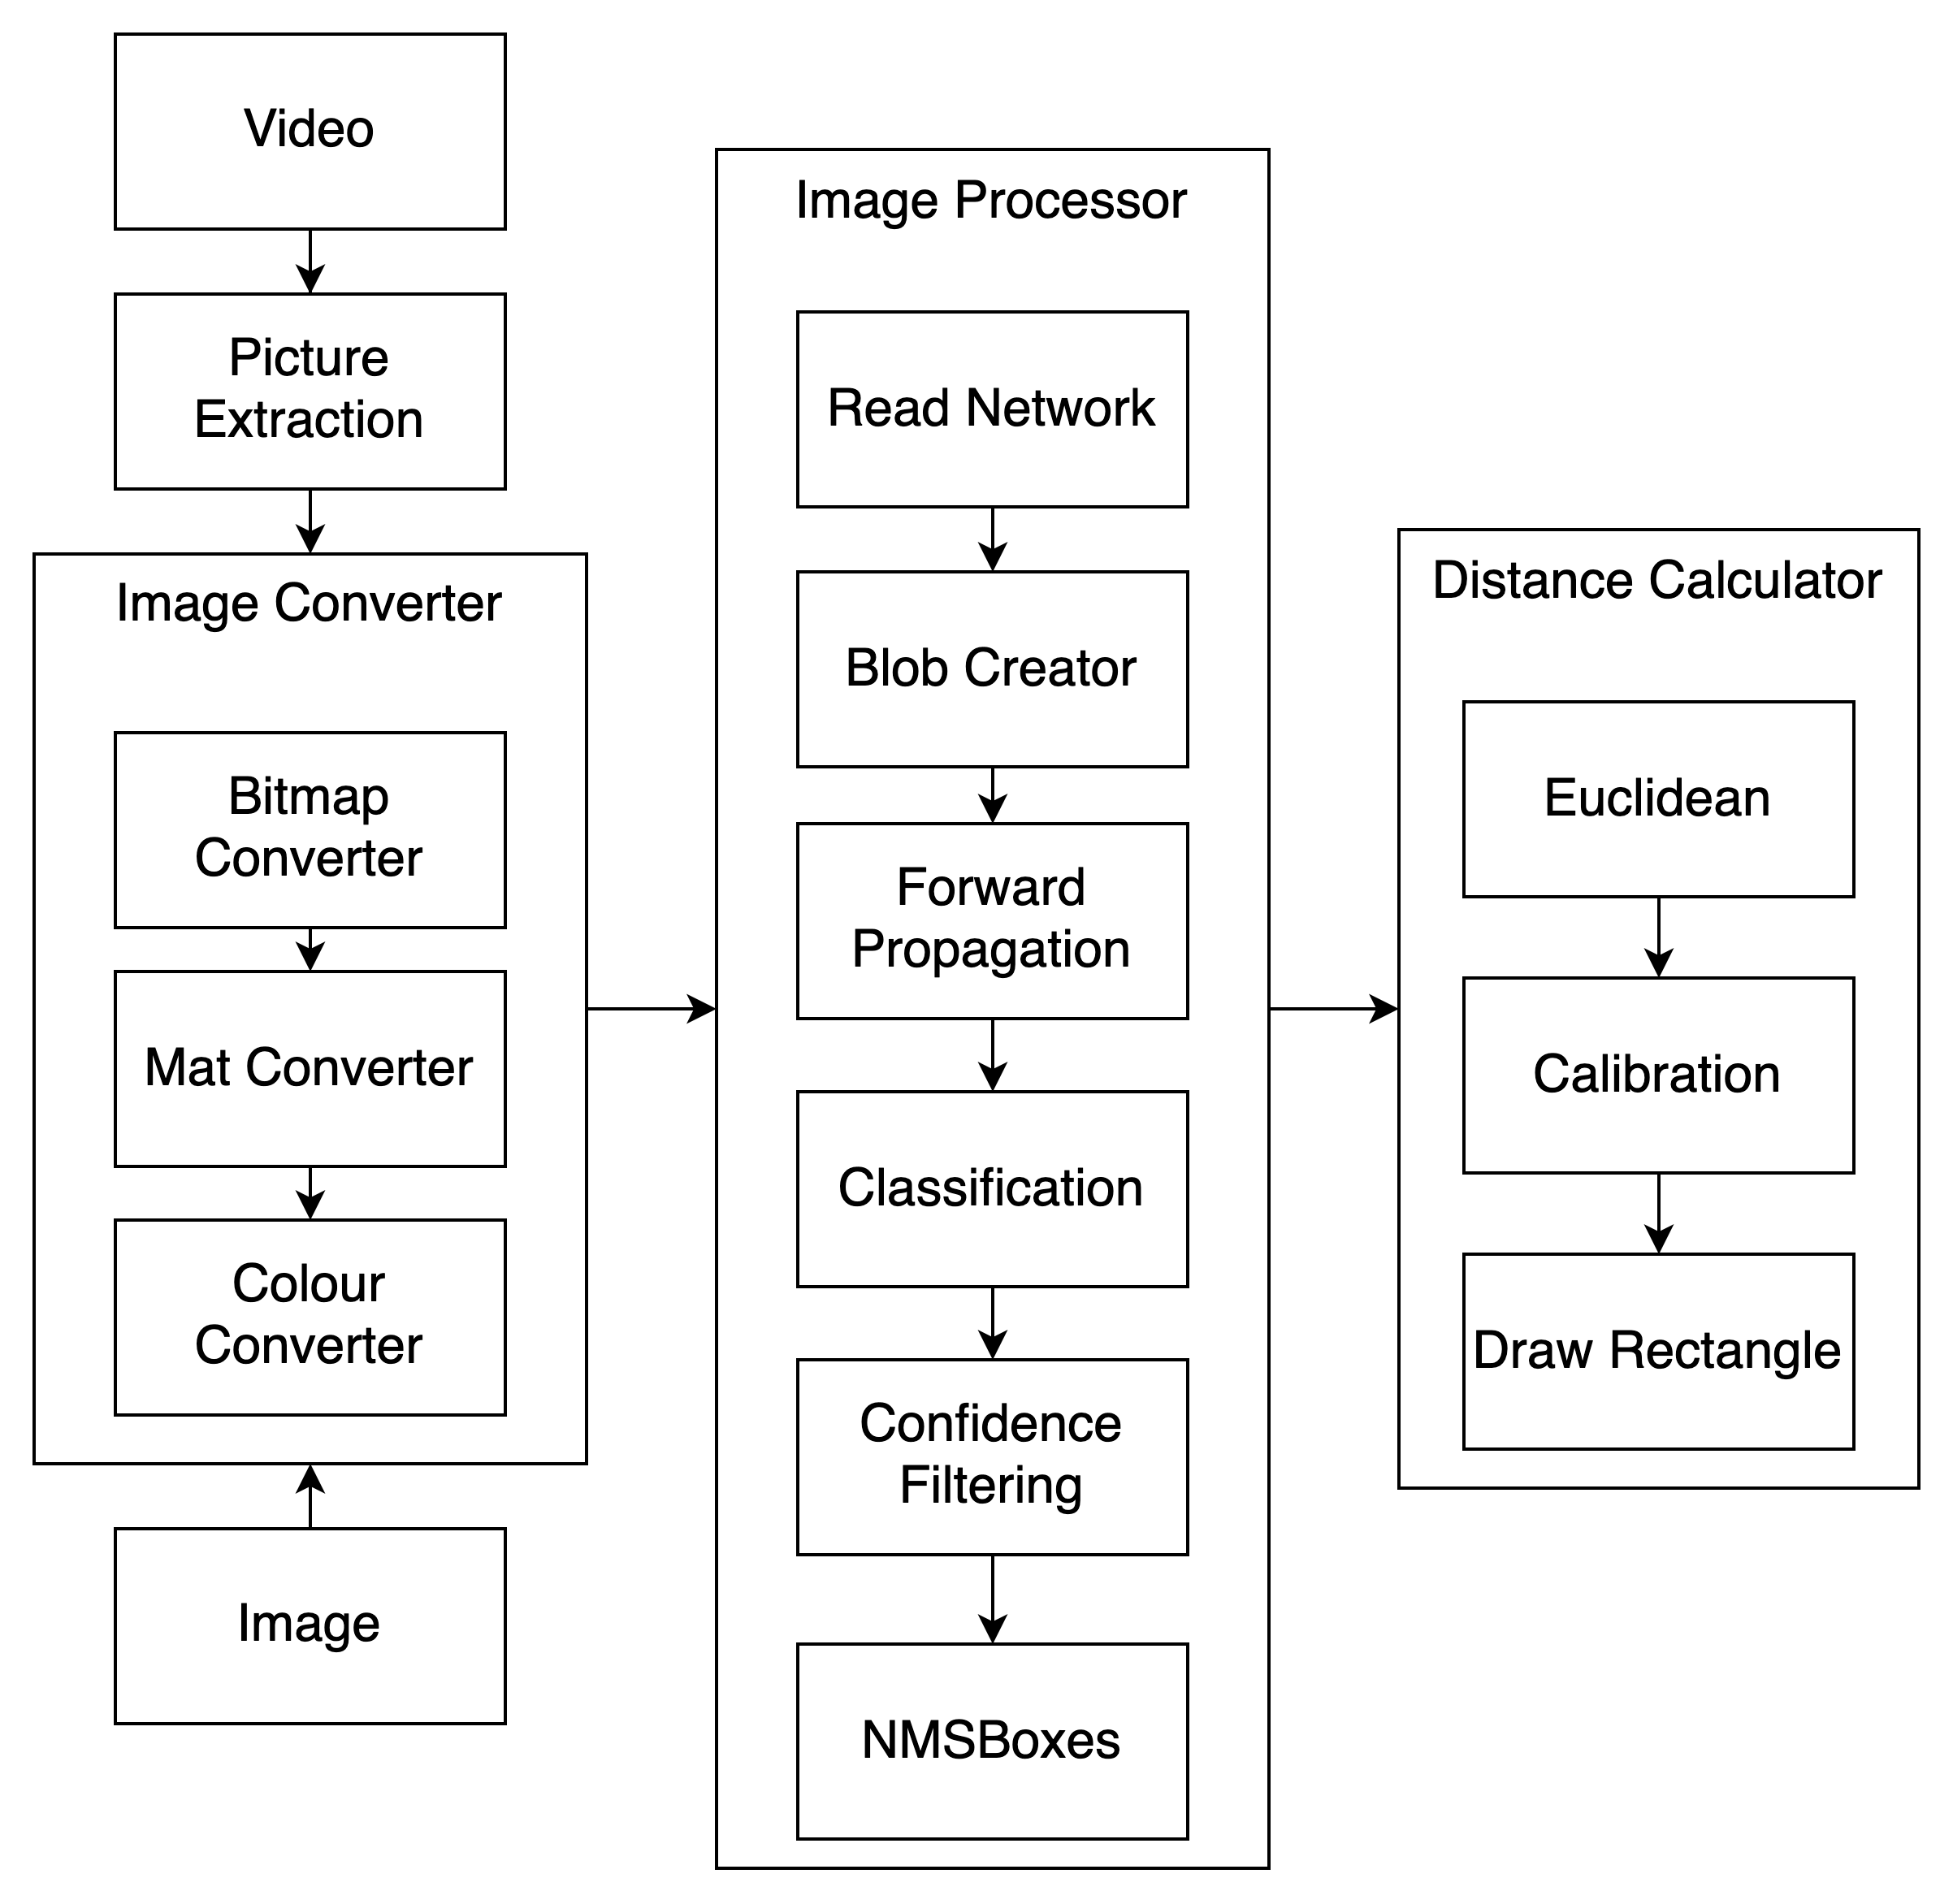
\includegraphics[width=5in]{images/chapter3/system-overview.png}
            \caption{System Overview Diagram}
            \label{systemOverview}
        \end{figure}

        -	How DNN is implemented
            - DNN is implemented by using OpenCV, and there are steps of processing
                - Video -> Image -> Mat
                - blobFromImage
                - setInput
                - net.forward (forward propagation)
                - determine classification and confidence(accuracy)
                - NMSBox
                - Calculate Distance

            - How to show processed frame from live stream?
            - insert image
        - pass social distancing = green, else = red

    \section{Parallelisation}
        -	Intro about parallelisation – How it works in Android
            - Thread vs ThreadPool
            - Handler
        -	Multithreading and Multicore
        -	System overview (Manager – Task – Runnable)
            - <Insert diagram>
        -	1 frame per 1 thread
            - <Insert diagram>

        \begin{figure}[!ht]
            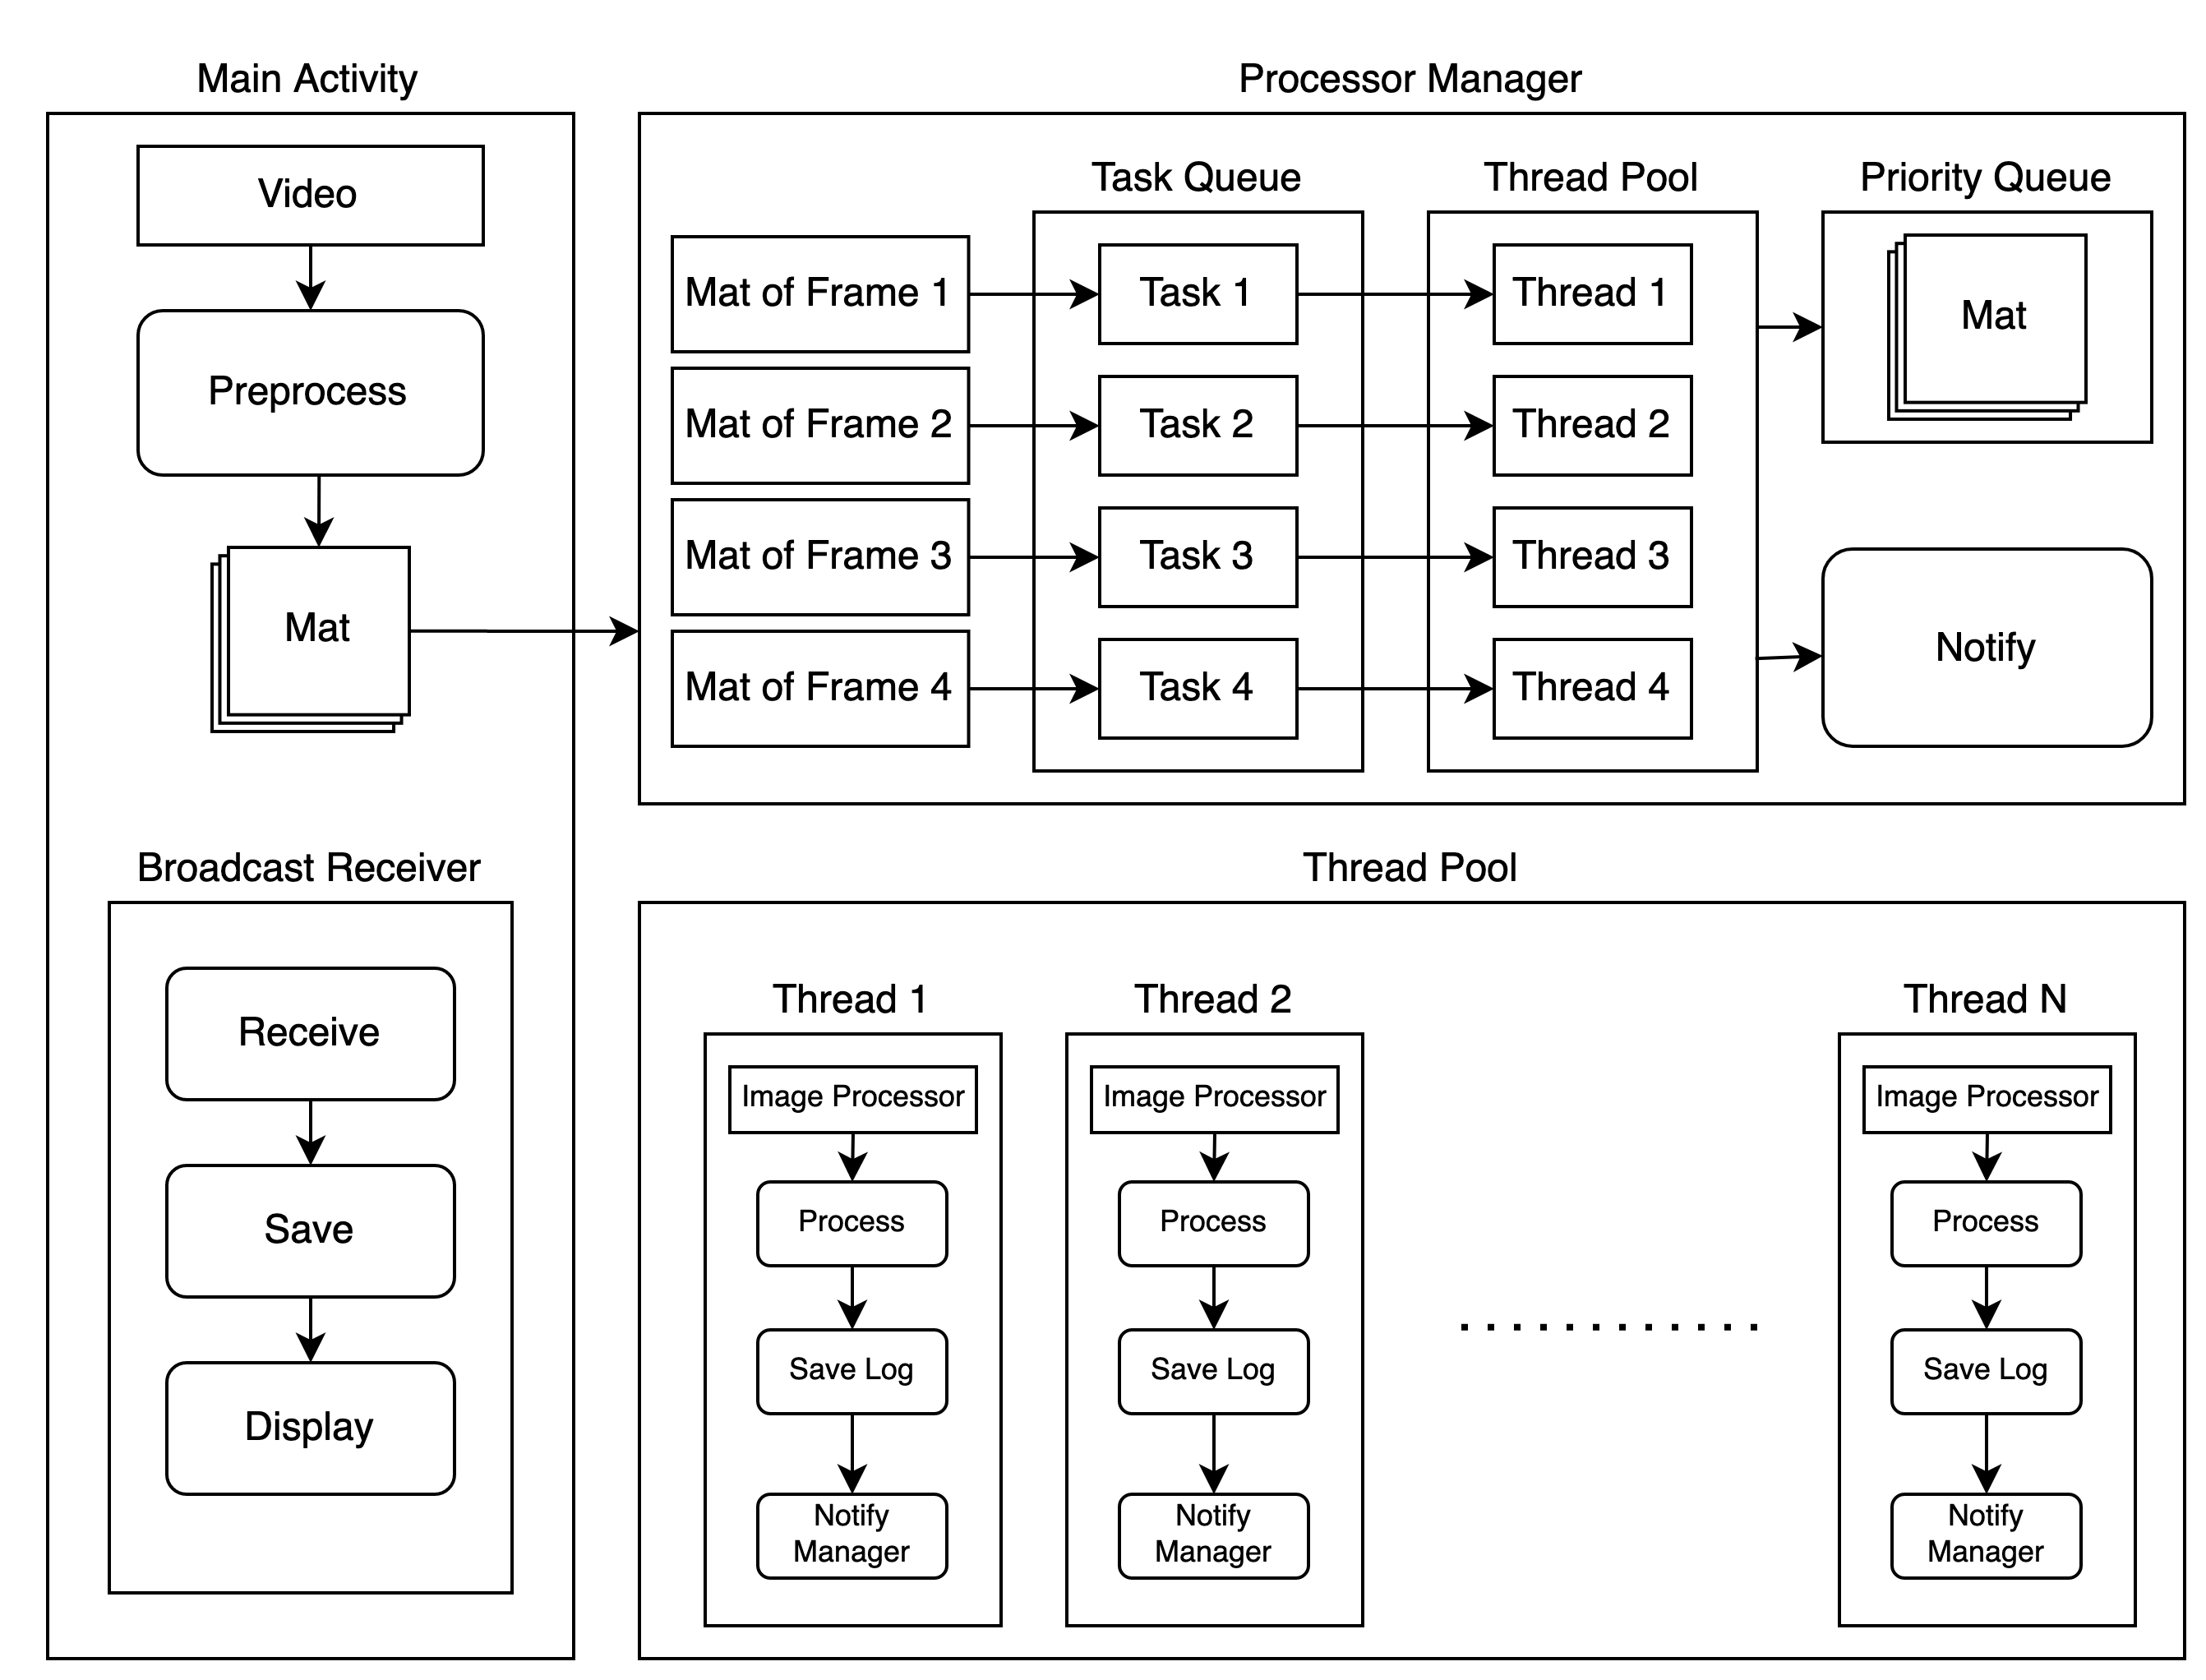
\includegraphics[width=6in]{images/chapter3/parallel.png}
            \caption{Parallel Computing Diagram}
            \label{systemOverview}
        \end{figure}

        \subsection{Multitheading with Java}
            -	How to implement
                - Using Java
                - Thread pool
                    <insert sample of code>
            -	Memory Management
                - Singleton Pattern
                - Static block
                    - Executed only once
                - Queue and recycling

        \subsection{Multitheading with C++}

